\documentclass[UTF8]{ctexart}
\usepackage{graphicx}
\usepackage{listings}


\title{Lab1 报告}
\author{唐灵\\519030910052\\F1903002}
\date{\today}

\begin{document}
    \maketitle
    \section{实验概览}
        总体来讲,本次实验可以分为四个子实验,即在利用pyton包的情况下,希望实现:
        \begin{enumerate}
            \item 通过url,模拟浏览器访问服务器的过程,抓取网络页面源代码信息,当然,这次主要针对的是html文档。
            \item 对页面源代码进行解析,生成dom树(将html文档表达为树结构),方便进行进一步的信息提取。
            \item 通过专门处理dom树的包(BeautifulSoup),来限定并遍历访问希望访问的节点。
            \item 通过正则表达式来匹配希望得到的特定信息,包括url,文本信息等。
            \item 最后一步不能算是实验,就是将得到的信息写入文件。
        \end{enumerate}
        以上的四个小实验,所幸不用我们自己来实现,只需要调用基于python的不同功能的封装完整的包,很多时候就是一句话就能够解决的事情。
    \section{实验环境}
        本次实验的所有代码在电类工程导论c课程中在课程方统一给定的“ee208”$Docker$容器中运行并实现,实验时间为2020年09月11日。
    \section{练习解决思路}
        \subsection{练习一的解决思路}
            练习一的解决思路跟在之前提到的实验概览中提到的一样,
            有一点值得提出来一下,那就是实验限定了我们应当舍去图像的链接,我的做法是,
            在遍历匹配得到了页面中所有的指定标签下的url的情况下,
            在中间边进行遍历的过程中先判定末尾四位结尾是否为:".jpg"或者是".png",
            通过验证的url再加入到我们的url集合当中,以上为两种常见的图片格式,应当能够满足大部分的需求。
        \subsection{练习二的解决思路}
            练习二中依然和练习一是大致相同的思路,只不过这次需求相反,我们需要图片,
            这和我们希望匹配页面中的网页链接的步骤可以同步运行,只需要稍微改变正则表达式的值:为“\^http.*.(jpg|png)\$”即可(上标应该在最前边,而不是在字母‘h’上)
            其他的做法完全一致。    
        \subsection{练习三的解决思路}
            针对问题三,与问题一二有两点不同:
            \begin{enumerate}
                \item 根据提示加入了消息头。
                \item 其次是需要找到多组符合条件的信息,而非单一信息。
            \end{enumerate}

            在按要求使用$.add\_headers()$的方法,通过传递字典,添加了消息头信息之后。
            认真观察网页,审查网页元素,发现我们希望找到的元素都在同一类标签$‘a’,\{“class”:“link-button”\}$之下,
            所以我们先通过bs找到这个标签,再进行遍历,每一次遍历过程处理这个节点下的子节点,提取信息,即可完成任务。
    \section{代码运行结果}
        \subsection{练习一的运行结果}
        练习一结果储存在result1.txt之中,每一行代表一个url,总共得到34条记录。
        \subsection{练习二的运行结果}
        练习二结果储存在result1.txt之中,每一行代表一个url,最终发现图片链接仅有.png格式,总过收获10条记录。
        \subsection{练习三的运行结果}
        练习三结果储存在result1.txt之中,每一行代表一组信息,总共得到了30组信息,部分截图如下
            \begin{figure}[ht]
                \centering
                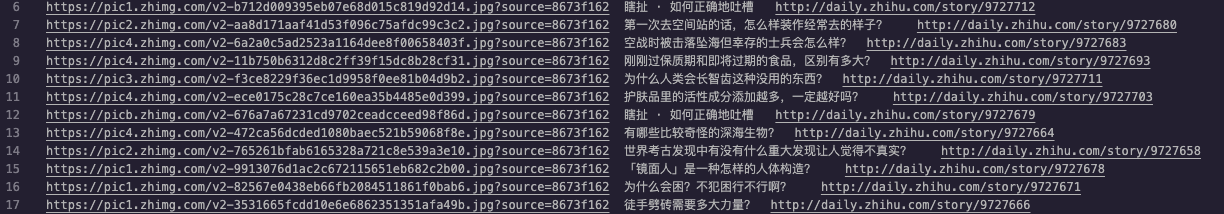
\includegraphics[scale=0.25]{img/result3_img.png}
                \caption{练习三程序运行结果}
            \end{figure}
        一段截图如下
    \section{分析与思考}
        本次实验进行了基本的网页爬取,没有什么很多好分析的,用包就完事儿了。

        值得一提的是本来想通过打印加头和不加信息头的结果来看一下反爬机制,结果发现真的就返回了正确的结果。
        消息头的添加也让我感到比较迷惑,通过这个方法添加消息头,从形式上来讲不就只能传递User-Agent的信息吗?
        网上查了查,还是有其他的方法是可以通过传递字典来进行消息头的添加的。
\end{document}